\documentclass[journal,12pt,twocolumn]{IEEEtran}
%\usepackage{setspace}
\usepackage{gensymb}
%\doublespacing
%\singlespacing

%\usepackage{graphicx}
%\usepackage{amssymb}
%\usepackage{relsize}
\usepackage[cmex10]{amsmath}
%\usepackage{amsthm}
%\interdisplaylinepenalty=2500
%\savesymbol{iint}
%\usepackage{txfonts}
%\restoresymbol{TXF}{iint}
%\usepackage{wasysym}
\usepackage{amsthm}
%\usepackage{iithtlc}
\usepackage{mathrsfs}
\usepackage{txfonts}
\usepackage{stfloats}
\usepackage{bm}
\usepackage{cite}
\usepackage{cases}
\usepackage{subfig}
%\usepackage{xtab}
\usepackage{longtable}
\usepackage{multirow}
%\usepackage{algorithm}
%\usepackage{algpseudocode}
\usepackage{enumitem}
\usepackage{mathtools}
\usepackage{tikz}
\usetikzlibrary{shapes,arrows}
\usepackage{circuitikz}
\usepackage{verbatim}
%\usepackage{tfrupee}
%\usepackage[breaklinks=true]{hyperref}
%\usepackage{stmaryrd}
%\usepackage{tkz-euclide} % loads  TikZ and tkz-base
%\usetkzobj{all}
%\usepackage{listings}
    \usepackage{color}                                            %%
    \usepackage{array}                                            %%
    \usepackage{longtable}                                        %%
    \usepackage{calc}                                             %%
    \usepackage{multirow}                                         %%
    \usepackage{hhline}                                           %%
    \usepackage{ifthen}                                           %%
  %optionally (for landscape tables embedded in another document): %%
    \usepackage{lscape}     
\usepackage{multicol}
\usepackage{chngcntr}
%\usepackage{enumerate}

%\usepackage{wasysym}
%\newcounter{MYtempeqncnt}
\DeclareMathOperator*{\Res}{Res}
%\renewcommand{\baselinestretch}{2}
\renewcommand\thesection{\arabic{section}}
\renewcommand\thesubsection{\thesection.\arabic{subsection}}
\renewcommand\thesubsubsection{\thesubsection.\arabic{subsubsection}}

\renewcommand\thesectiondis{\arabic{section}}
\renewcommand\thesubsectiondis{\thesectiondis.\arabic{subsection}}
\renewcommand\thesubsubsectiondis{\thesubsectiondis.\arabic{subsubsection}}

% correct bad hyphenation here
\hyphenation{op-tical net-works semi-conduc-tor}
\def\inputGnumericTable{}                                 %%

%\lstset{
%language=C,
%frame=single, 
%breaklines=true,
%columns=fullflexible
%}
%\lstset{
%language=tex,
%frame=single, 
%breaklines=true
%}

\begin{document}
%


\newtheorem{theorem}{Theorem}[section]
\newtheorem{problem}{Problem}
\newtheorem{proposition}{Proposition}[section]
\newtheorem{lemma}{Lemma}[section]
\newtheorem{corollary}[theorem]{Corollary}
\newtheorem{example}{Example}[section]
\newtheorem{definition}[problem]{Definition}
%\newtheorem{thm}{Theorem}[section] 
%\newtheorem{defn}[thm]{Definition}
%\newtheorem{algorithm}{Algorithm}[section]
%\newtheorem{cor}{Corollary}
\newcommand{\BEQA}{\begin{eqnarray}}
\newcommand{\EEQA}{\end{eqnarray}}
\newcommand{\define}{\stackrel{\triangle}{=}}
\bibliographystyle{IEEEtran}
%\bibliographystyle{ieeetr}
\providecommand{\mbf}{\mathbf}
\providecommand{\pr}[1]{\ensuremath{\Pr\left(#1\right)}}
\providecommand{\qfunc}[1]{\ensuremath{Q\left(#1\right)}}
\providecommand{\sbrak}[1]{\ensuremath{{}\left[#1\right]}}
\providecommand{\lsbrak}[1]{\ensuremath{{}\left[#1\right.}}
\providecommand{\rsbrak}[1]{\ensuremath{{}\left.#1\right]}}
\providecommand{\brak}[1]{\ensuremath{\left(#1\right)}}
\providecommand{\lbrak}[1]{\ensuremath{\left(#1\right.}}
\providecommand{\rbrak}[1]{\ensuremath{\left.#1\right)}}
\providecommand{\cbrak}[1]{\ensuremath{\left\{#1\right\}}}
\providecommand{\lcbrak}[1]{\ensuremath{\left\{#1\right.}}
\providecommand{\rcbrak}[1]{\ensuremath{\left.#1\right\}}}
\theoremstyle{remark}
\newtheorem{rem}{Remark}
\newcommand{\sgn}{\mathop{\mathrm{sgn}}}
\providecommand{\abs}[1]{\left\vert#1\right\vert}
\providecommand{\res}[1]{\Res\displaylimits_{#1}} 
\providecommand{\norm}[1]{\left\lVert#1\right\rVert}
%\providecommand{\norm}[1]{\lVert#1\rVert}
\providecommand{\mtx}[1]{\mathbf{#1}}
\providecommand{\mean}[1]{E\left[ #1 \right]}
\providecommand{\fourier}{\overset{\mathcal{F}}{ \rightleftharpoons}}
%\providecommand{\hilbert}{\overset{\mathcal{H}}{ \rightleftharpoons}}
\providecommand{\system}{\overset{\mathcal{H}}{ \longleftrightarrow}}
	%\newcommand{\solution}[2]{\textbf{Solution:}{#1}}
\newcommand{\solution}{\noindent \textbf{Solution: }}
\newcommand{\cosec}{\,\text{cosec}\,}
\providecommand{\dec}[2]{\ensuremath{\overset{#1}{\underset{#2}{\gtrless}}}}
\newcommand{\myvec}[1]{\ensuremath{\begin{pmatrix}#1\end{pmatrix}}}
\newcommand{\mydet}[1]{\ensuremath{\begin{vmatrix}#1\end{vmatrix}}}
%\numberwithin{equation}{section}
\numberwithin{equation}{subsection}
%\numberwithin{problem}{section}
%\numberwithin{definition}{section}
\makeatletter
\@addtoreset{figure}{problem}
\makeatother
\let\StandardTheFigure\thefigure
\let\vec\mathbf
%\renewcommand{\thefigure}{\theproblem.\arabic{figure}}
\renewcommand{\thefigure}{\theproblem}
%\setlist[enumerate,1]{before=\renewcommand\theequation{\theenumi.\arabic{equation}}
%\counterwithin{equation}{enumi}
%\renewcommand{\theequation}{\arabic{subsection}.\arabic{equation}}
\def\putbox#1#2#3{\makebox[0in][l]{\makebox[#1][l]{}\raisebox{\baselineskip}[0in][0in]{\raisebox{#2}[0in][0in]{#3}}}}
     \def\rightbox#1{\makebox[0in][r]{#1}}
     \def\centbox#1{\makebox[0in]{#1}}
     \def\topbox#1{\raisebox{-\baselineskip}[0in][0in]{#1}}
     \def\midbox#1{\raisebox{-0.5\baselineskip}[0in][0in]{#1}}
\vspace{3cm}
\title{
	\logo{
Control Systems
	}
}
\author{ G V V Sharma$^{*}$% <-this % stops a space
	\thanks{*The author is with the Department
		of Electrical Engineering, Indian Institute of Technology, Hyderabad
		502285 India e-mail:  gadepall@iith.ac.in. All content in this manual is released under GNU GPL.  Free and open source.}
	
}	
%\title{
%	\logo{Matrix Analysis through Octave}{\begin{center}\includegraphics[scale=.24]{tlc}\end{center}}{}{HAMDSP}
%}
% paper title
% can use linebreaks \\ within to get better formatting as desired
%\title{Matrix Analysis through Octave}
%
%
% author names and IEEE memberships
% note positions of commas and nonbreaking spaces ( ~ ) LaTeX will not break
% a structure at a ~ so this keeps an author's name from being broken across
% two lines.
% use \thanks{} to gain access to the first footnote area
% a separate \thanks must be used for each paragraph as LaTeX2e's \thanks
% was not built to handle multiple paragraphs
%
%\author{<-this % stops a space
%\thanks{}}
%}
% note the % following the last \IEEEmembership and also \thanks - 
% these prevent an unwanted space from occurring between the last author name
% and the end of the author line. i.e., if you had this:
% 
% \author{....lastname \thanks{...} \thanks{...} }
%                     ^------------^------------^----Do not want these spaces!
%
% a space would be appended to the last name and could cause every name on that
% line to be shifted left slightly. This is one of those "LaTeX things". For
% instance, "\textbf{A} \textbf{B}" will typeset as "A B" not "AB". To get
% "AB" then you have to do: "\textbf{A}\textbf{B}"
% \thanks is no different in this regard, so shield the last } of each \thanks
% that ends a line with a % and do not let a space in before the next \thanks.
% Spaces after \IEEEmembership other than the last one are OK (and needed) as
% you are supposed to have spaces between the names. For what it is worth,
% this is a minor point as most people would not even notice if the said evil
% space somehow managed to creep in.
% The paper headers
%\markboth{Journal of \LaTeX\ Class Files,~Vol.~6, No.~1, January~2007}%
%{Shell \MakeLowercase{\textit{et al.}}: Bare Demo of IEEEtran.cls for Journals}
% The only time the second header will appear is for the odd numbered pages
% after the title page when using the twoside option.
% 
% *** Note that you probably will NOT want to include the author's ***
% *** name in the headers of peer review papers.                   ***
% You can use \ifCLASSOPTIONpeerreview for conditional compilation here if
% you desire.
% If you want to put a publisher's ID mark on the page you can do it like
% this:
%\IEEEpubid{0000--0000/00\$00.00~\copyright~2007 IEEE}
% Remember, if you use this you must call \IEEEpubidadjcol in the second
% column for its text to clear the IEEEpubid mark.
% make the title area
%\maketitle
\newpage
\tableofcontents
\bigskip
\renewcommand{\thefigure}{\theenumi}
\renewcommand{\thetable}{\theenumi}
%\renewcommand{\theequation}{\theenumi}
%\begin{abstract}
%%\boldmath
%In this letter, an algorithm for evaluating the exact analytical bit error rate  (BER)  for the piecewise linear (PL) combiner for  multiple relays is presented. Previous results were available only for upto three relays. The algorithm is unique in the sense that  the actual mathematical expressions, that are prohibitively large, need not be explicitly obtained. The diversity gain due to multiple relays is shown through plots of the analytical BER, well supported by simulations. 
%
%\end{abstract}
% IEEEtran.cls defaults to using nonbold math in the Abstract.
% This preserves the distinction between vectors and scalars. However,
% if the journal you are submitting to favors bold math in the abstract,
% then you can use LaTeX's standard command \boldmath at the very start
% of the abstract to achieve this. Many IEEE journals frown on math
% in the abstract anyway.
% Note that keywords are not normally used for peerreview papers.
%\begin{IEEEkeywords}
%Cooperative diversity, decode and forward, piecewise linear
%\end{IEEEkeywords}
% For peer review papers, you can put extra information on the cover
% page as needed:
% \ifCLASSOPTIONpeerreview
% \begin{center} \bfseries EDICS Category: 3-BBND \end{center}
% \fi
%
% For peerreview papers, this IEEEtran command inserts a page break and
% creates the second title. It will be ignored for other modes.
%\IEEEpeerreviewmaketitle
\begin{abstract}
This manual is an introduction to control systems based on GATE problems.Links to sample Python codes are available in the text.  
\end{abstract}
Download python codes using 
%\begin{lstlisting}
%svn co https://github.com/gadepall/school/trunk/control/codes
%\end{lstlisting}
%\section{Bode Plot}
%\begin{enumerate}[label=\thesection.\arabic*.,ref=\thesection.\theenumi]
%\numberwithin{equation}{enumi}
%\input{./chapters/ee18btech11001.tex}
%\end{enumerate}
\section{Stability}
\section{Routh Hurwitz Criterion}
For a feedback transconductance amplifier in Fig \ref{fig:ee18btech11041_fig1}, derive an approximate expression for the closed loop transconductance T for the case of GH $\gg$1. Hence select a value of $R_2$ to obtain T=100 mA/V. If Q is biased to obtain $g_m$ = 1mA/V, specify  the value of the gian $\mu$ of the differential amplifier to obtain an amount of feedback of 60 dB. If Q has $r_o$ = 50 k$\ohm$ find the $R_{out}$.

\begin{figure}[!ht]
	\begin{center}
		\resizebox{\columnwidth}{!}{\ctikzset{tripoles/mos style/arrows}
\usetikzlibrary{decorations.markings}
\begin{circuitikz}
\ctikzset{bipoles/length=1cm}

\draw 
(0,0) node[op amp,yscale=-1.0] (opamp) {\rotatebox{180}{\reflectbox{$\mu$}}}
(1.5,0) node[nmos,](Q){}
(opamp.+) (-0.85, +0.35) -- (-3, +0.35) to [V=$V_s$] (-3,-1) to (-3,-1) node[ground]{}
(opamp.-) (-0.85, -0.35) -- (-0.85, -1.7) to [R=$R_3$] (-0.85,-4) to (-0.85,-4) node[ground]{}
(opamp.-) (-0.85, -0.35) -- (-0.85, -1.7) to [R=$R_2$] (1.5,-1.7) to (1.5,-1.7) 
(1.5,-0.5) to (1.5, -1.7) to [R=$R_1$] (1.5,-4) node[ground]{}

node at(-1.2,-1.7){$V_f$}
node at(1.8,-0.6){$I_o$}
node at (-0.2,-3.3){$100\ohm$}
node at (2.2,-3.3){$100\ohm$}
 ;



\draw[thick,->,>=stealth] (1.5,-0.9) -- (1.5,-1);

\draw[thick,->,>=stealth] (Q.D);


\end{circuitikz}
}
	\end{center}
\caption{Complete Circuit}
\label{fig:ee18btech11041_fig1}
\end{figure}
\begin{enumerate}[label=\arabic*.,ref=\theenumi]
\numberwithin{equation}{enumi}
\numberwithin{figure}{enumi}

\item Draw the small signal model for Fig. \ref{fig:ee18btech11041_fig1}
%
\\
\solution See Fig. \ref{fig:ee18btech11041_fig2}



\begin{figure}[!ht]
	\begin{center}
		\resizebox{\columnwidth}{!}{\begin{circuitikz}
\ctikzset{bipoles/length=1cm}
\draw
(0,0) to[short,*-*] (1,0){}
(0.5,0) -- (0.5,-0.5) to[R, l_=$R_{id}$] (0.5,-1.5) (0.5,-1.5)--(0.5,-3.5) 
(0.5,-3.5) to [R=$R_3$] (0.5,-4.5){}
(0.5,-4.5) node[ground]{}

(0.5,-3) -- (2.5,-3) to [R=$R_{2}$] (3.5,-3) -- (5.5,-3) 

(2,0) to[R=$r_{01}$,*-*] (4,0){}
(2,0) to[cV=$\mu V_i$] (2,-2)  {}
(2,-2) node[ground]{}
(5.5,0) to[I=$g_{m}V_{gs}$] (5.5,-2){}
(5.5,0)--((5.5,1) --(6,1) node[ground]{}
(5.5,0) -- (7,0) to[R=$r_{0}$] (7,-2) -- (5.5,-2){}
(5.5,-2) to[short, i = $I_{o}$] (5.5,-3.5) to[R=$R_1$] (5.5,-4.5) node[ground]{}


node at(4.1,-1) {$V_{gs}$}

node at(4.1,-0.2) {$+$}
node at(4.1,-2) {$-$}
node at(0,0.25) {$V_s$}

node at(0.7,-0.3) {$+$}
node at(0.7,-1.7) {$-$}
node at(0.9,-1.2) {$V_i$}

;\end{circuitikz}}
	\end{center}
\caption{Small signal model}
\label{fig:ee18btech11041_fig2}
\end{figure}

\item Draw the block diagram and the transconductance freedback model.
\\
\solution See Figs. \ref{fig:ee18btech11041_fig3} and \ref{fig:ee18btech11041_fig3}

\begin{figure}[!ht]
	\begin{center}
		\resizebox{\columnwidth}{!}{\tikzstyle{block} = [draw, rectangle, 
    minimum height=1.25em, minimum width=2.5em]
\tikzstyle{sum} = [draw, circle, node distance=1cm]
\tikzstyle{input} = [coordinate]
\tikzstyle{output} = [coordinate]
\tikzstyle{pinstyle} = [pin edge={to-,thin,black}]


\begin{tikzpicture}[auto, node distance=2.5cm,>=latex']
   
    \node [input, name=input] {};
    \node [sum, right of=input] (sum) {};
    \node [block, right of=sum] (controller) {$G$};
    
    \node [output, right of=controller] (output) {};
    \node [block, below of=controller] (measurements) {$H$};

   \draw [draw,->] (input) -- node[pos=0.99] {$+$} node {$V_{s}$} (sum);
    \draw [->] (sum) -- node {$V_{i}$} (controller);
    \draw [->] (controller) -- node [name=y] {$I_{o}$}(output);
    \draw [->] (y) |- (measurements);
    \draw [->] (measurements) -| node[pos=0.99] {$-$} node [near end] {$V_{f}$} (sum);
\end{tikzpicture}}
	\end{center}
\caption{Block Diagram}
\label{fig:ee18btech11041_fig3}
\end{figure}

\begin{figure}[!ht]
	\begin{center}
		\resizebox{\columnwidth}{!}{\begin{circuitikz}[american]
\usetikzlibrary{positioning, fit, calc}
\draw (0,0)to [voltage source,v=$V_s$]++(0,-2)
(0,0)to[R=$R_s$,i=$I_i$](6,0)to[R,v^>=${V}_i$,*-]++(0,-2)--++(-2,0)--++(0,-2)--++(4,0)to[controlled voltage source=$HI_o$]++(0,-2)--++(-6,0)--++(0,4)--++(-2,0)--(0,-2);
\draw (10,0) to [controlled current source=$GV_i$]++(0,-2)
(10,0)--(12,0)to[R=$R_o$]++(0,-2)--(14,-2)--(14,-4)--(12,-4)--(12,-6)--++(4,0)--++(0,4)--++(2,0)to[R=$R_L$]++(0,2)to [short,i=$I_o$](12,0)
(10,-2)--(12,-2)
(5,0)coordinate(left)
(5,-2)coordinate(bottoml)
(13,0)coordinate(right)
(13,-2)coordinate(bottomr)
node[fit=(left)(right)(bottoml)(bottomr),draw, dashed, label={amplifier circuit},inner sep=10pt] {}
(5,-4)coordinate(left1)
(5,-6)coordinate(bottoml1)
(13,-4)coordinate(right1)
(13,-6)coordinate(bottomr1)
node[fit=(left1)(right1)(bottoml1)(bottomr1),draw, dashed, label={feedback circuit},inner sep=10pt] {}
(5,-1)node[label={right:$R_i$}]{}
(2,-2)to [open, v^<=${V}_f$,*-]++(2,0)

;\end{circuitikz}}
	\end{center}
\caption{Transconductance amplifier}
\label{fig:ee18btech11041_fig4}
\end{figure}
%
\item  Draw the feedback circuit for $H$ and compute it.
\\
\solution From Fig. \ref{fig:ee18btech11041_fig5}, using current division,
%
\begin{align}
V_f &= I_o \times \frac{R_1}{R_1+R_2+R_3}\times R_3
\\
\implies 
H &= \frac{V_f}{I_o}
\\
&= \frac{R_1 R_3}{R_1+R_2+R_3}
\end{align}
\begin{figure}[!ht]
	\begin{center}
		\resizebox{\columnwidth}{!}{\begin{circuitikz}
\ctikzset{bipoles/length=1cm}

\draw 
(0,0)  to[R=$R_2$] (3,0) to[R=$R_1$] (3,-2) node[ground]{}
(0,0) to [R=$R_3$](0,-2)  (0,-2) node[ground]{}
(3,0) -- (4,0){}
(4,-2) node[ground]{}
(4,-2) to[I=$I_o$] (4,0){}

node at(0,0.3){$V_f$}
node at(3,0.3){$V_x$}


;\end{circuitikz}}
	\end{center}
\caption{Feedback Circuit}
\label{fig:ee18btech11041_fig5}
\end{figure}

\item For $GH \gg 1,T = 100$ mA/V, find $H$ and $R_2$.
\\
\solution 

\begin{align}
    T &\approx \frac{1}{H}
    \label{eq:ee18btech11041_eq6}
\\
     &= \frac{R_1+R_2+R_3}{R_1 R_3}
\\
\implies     R_2 &= 800 \ohm \quad \text{and}
    \label{eq:ee18btech11041_eq7}
\\
 H &=10
\end{align}

\item Find $R_{11}$ and $R_{22}$ in Fig. \ref{fig:ee18btech11041_fig6}


\begin{figure}[!ht]
	\begin{center}
		\resizebox{\columnwidth}{!}{\begin{circuitikz}[american]
\usetikzlibrary{positioning, fit, calc}
\draw (0,0)to [voltage source,v=$V_i$]++(0,-2)to[R=$R_{11}$]++(6,0)
(0,0)to[short](6,0);
\draw (8,-1)node[draw,minimum width=4cm,minimum height=4cm] (load) {Gain Block}(8,0)
(10,0)--++(6,0)to[short]++(0,-2)to [R=$R_{22}$,i<=$I_O$](10,-2)
;
\end{circuitikz}}
	\end{center}
\caption{Block Diagram of G}
\label{fig:ee18btech11041_fig6}
\end{figure}
\solution  From Fig. \ref{fig:ee18btech11041_fig5},
%
\begin{align}
    R_{11} = (R_2+R_1)\parallel R_3
\end{align}

\begin{align}
    R_{22} = (R_2+R_3) \parallel R_1
\end{align}

\item Draw the equivalent circuit for $G$ and find it.
\\
\solution 
\begin{figure}[!ht]
	\begin{center}
		\resizebox{\columnwidth}{!}{\begin{circuitikz}
\ctikzset{bipoles/length=1cm}
\draw
(0,0) to[short] (2.5,0){}
(0,0) to [V=$V_i$] (0,-3) {}
(0,-3) node[ground]{}
(2.5,0) -- (2.5,-0.5) to[R, l_=$R_{id}\xrightarrow{}\infty$] (2.5,-1.5) {} 
(2.5,-1.5) to [R=$R_{11}$] (2.5,-3){}
(2.5,-3) node[ground]{}


(4,0) to[R=$r_{01}$,*-*] (6,0){}
(4,0) to[cV=$\mu V_i$] (4,-3)  {}
(4,-3) node[ground]{}
(7,0) to[I=$g_{m}V_{gs}$] (7,-2){}
(7,0)--((7,1) --(7.5,1) node[ground]{}
(7,0) -- (8.5,0) to[R=$r_{0}$] (8.5,-2) -- (7,-2){}
(7,-2) to[short, i = $I_{o}$] (7,-3) -- (7,-3.5) to[R=$R_{22}$] (7,-4.5) -- (7,-5) node[ground]{}


node at(6.1,-2) {$V_{gs}$}

node at(6.1,-0.2) {$+$}
node at(6.1,-2.5) {$-$}

node at(7.5,-3.2) {$V_x$}
node at(2.7,-0.3) {$+$}
node at(2.7,-1.7) {$-$}
node at(2.9,-1.2) {$V_i$}

;\end{circuitikz}}
	\end{center}
\caption{Gain equivalent circuit}
\label{fig:ee18btech11041_fig7}
\end{figure}
\begin{align}
    G = \frac{I_o}{V_i} 
    \label{eq;eq8}
\end{align}

From Fig. \ref{fig:ee18btech11041_fig7} we can see that
 
\begin{align}
    V_{gs} = \mu V_i - V_x
    \label{eq;eq9}
\end{align}

\begin{align}
    g_mV_{gs} - \frac{V_x}{r_o} = I_o
    \label{eq;eq10}
\end{align}

From equations \ref{eq;eq9} to \ref{eq;eq10}
\begin{align}
    G = \frac{I_o}{V_i} = \frac{g_m \mu r_o}{r_o + (1+g_m r_o)((R_2+R_3) \parallel R_1) }
    \label{eq:ee18btech11041_eq11}
\end{align}
\item If GH = 60dB, find $\mu$.
\\
\solution 
\begin{align}
    20\log_{10} GH &= 60 
    \label{eq:ee18btech11041_eq12}
\\
\implies G&=100
\end{align}

Substituting the values in the Eq. \ref{eq:ee18btech11041_eq11}
\begin{align}
    \mu = 109180
\end{align}
%
%\item Find $R_{out}$.
%\\
%\solution 
%For output reistance,
%\begin{align}
%    R_o = r_o + g_m r_o((R_2+R_3) \parallel R_1) + ((R_2+R_3) \parallel R_1)    
%    \label{eq:ee18btech11041_eq13}
%\end{align}
%Substituting the values in Eq.\ref{eq:ee18btech11041_eq13} 
%\begin{align}
%    R_o=54.59k\ohm
%\end{align}
%\begin{align}
%R_{out} = R_o(1+GH)    
%\end{align}
%
%$\implies$  $R_{out}$ = 54.64 M$\ohm$


%\begin{table}[!ht]
%\centering
%%%%%%%%%%%%%%%%%%%%%%%%%%%%%%%%%%%%%%%%%%%%%%%%%%%%%%%%%%%%%%%%%%%%%%%
%%                                                                  %%
%%  This is the header of a LaTeX2e file exported from Gnumeric.    %%
%%                                                                  %%
%%  This file can be compiled as it stands or included in another   %%
%%  LaTeX document. The table is based on the longtable package so  %%
%%  the longtable options (headers, footers...) can be set in the   %%
%%  preamble section below (see PRAMBLE).                           %%
%%                                                                  %%
%%  To include the file in another, the following two lines must be %%
%%  in the including file:                                          %%
%%        \def\inputGnumericTable{}                                 %%
%%  at the beginning of the file and:                               %%
%%        \input{name-of-this-file.tex}                             %%
%%  where the table is to be placed. Note also that the including   %%
%%  file must use the following packages for the table to be        %%
%%  rendered correctly:                                             %%
%%    \usepackage[latin1]{inputenc}                                 %%
%%    \usepackage{color}                                            %%
%%    \usepackage{array}                                            %%
%%    \usepackage{longtable}                                        %%
%%    \usepackage{calc}                                             %%
%%    \usepackage{multirow}                                         %%
%%    \usepackage{hhline}                                           %%
%%    \usepackage{ifthen}                                           %%
%%  optionally (for landscape tables embedded in another document): %%
%%    \usepackage{lscape}                                           %%
%%                                                                  %%
%%%%%%%%%%%%%%%%%%%%%%%%%%%%%%%%%%%%%%%%%%%%%%%%%%%%%%%%%%%%%%%%%%%%%%



%%  This section checks if we are begin input into another file or  %%
%%  the file will be compiled alone. First use a macro taken from   %%
%%  the TeXbook ex 7.7 (suggestion of Han-Wen Nienhuys).            %%
\def\ifundefined#1{\expandafter\ifx\csname#1\endcsname\relax}


%%  Check for the \def token for inputed files. If it is not        %%
%%  defined, the file will be processed as a standalone and the     %%
%%  preamble will be used.                                          %%
\ifundefined{inputGnumericTable}

%%  We must be able to close or not the document at the end.        %%
	\def\gnumericTableEnd{\end{document}}


%%%%%%%%%%%%%%%%%%%%%%%%%%%%%%%%%%%%%%%%%%%%%%%%%%%%%%%%%%%%%%%%%%%%%%
%%                                                                  %%
%%  This is the PREAMBLE. Change these values to get the right      %%
%%  paper size and other niceties.                                  %%
%%                                                                  %%
%%%%%%%%%%%%%%%%%%%%%%%%%%%%%%%%%%%%%%%%%%%%%%%%%%%%%%%%%%%%%%%%%%%%%%

	\documentclass[12pt%
			  %,landscape%
                    ]{report}
       \usepackage[latin1]{inputenc}
       \usepackage{fullpage}
       \usepackage{color}
       \usepackage{array}
       \usepackage{longtable}
       \usepackage{calc}
       \usepackage{multirow}
       \usepackage{hhline}
       \usepackage{ifthen}

	\begin{document}


%%  End of the preamble for the standalone. The next section is for %%
%%  documents which are included into other LaTeX2e files.          %%
\else

%%  We are not a stand alone document. For a regular table, we will %%
%%  have no preamble and only define the closing to mean nothing.   %%
    \def\gnumericTableEnd{}

%%  If we want landscape mode in an embedded document, comment out  %%
%%  the line above and uncomment the two below. The table will      %%
%%  begin on a new page and run in landscape mode.                  %%
%       \def\gnumericTableEnd{\end{landscape}}
%       \begin{landscape}


%%  End of the else clause for this file being \input.              %%
\fi

%%%%%%%%%%%%%%%%%%%%%%%%%%%%%%%%%%%%%%%%%%%%%%%%%%%%%%%%%%%%%%%%%%%%%%
%%                                                                  %%
%%  The rest is the gnumeric table, except for the closing          %%
%%  statement. Changes below will alter the table's appearance.     %%
%%                                                                  %%
%%%%%%%%%%%%%%%%%%%%%%%%%%%%%%%%%%%%%%%%%%%%%%%%%%%%%%%%%%%%%%%%%%%%%%

\providecommand{\gnumericmathit}[1]{#1} 
%%  Uncomment the next line if you would like your numbers to be in %%
%%  italics if they are italizised in the gnumeric table.           %%
%\renewcommand{\gnumericmathit}[1]{\mathit{#1}}
\providecommand{\gnumericPB}[1]%
{\let\gnumericTemp=\\#1\let\\=\gnumericTemp\hspace{0pt}}
 \ifundefined{gnumericTableWidthDefined}
        \newlength{\gnumericTableWidth}
        \newlength{\gnumericTableWidthComplete}
        \newlength{\gnumericMultiRowLength}
        \global\def\gnumericTableWidthDefined{}
 \fi
%% The following setting protects this code from babel shorthands.  %%
 \ifthenelse{\isundefined{\languageshorthands}}{}{\languageshorthands{english}}
%%  The default table format retains the relative column widths of  %%
%%  gnumeric. They can easily be changed to c, r or l. In that case %%
%%  you may want to comment out the next line and uncomment the one %%
%%  thereafter                                                      %%
\providecommand\gnumbox{\makebox[0pt]}
%%\providecommand\gnumbox[1][]{\makebox}

%% to adjust positions in multirow situations                       %%
\setlength{\bigstrutjot}{\jot}
\setlength{\extrarowheight}{\doublerulesep}

%%  The \setlongtables command keeps column widths the same across  %%
%%  pages. Simply comment out next line for varying column widths.  %%
\setlongtables

\setlength\gnumericTableWidth{%
	53pt+%
	93pt+%
0pt}
\def\gumericNumCols{2}
\setlength\gnumericTableWidthComplete{\gnumericTableWidth+%
         \tabcolsep*\gumericNumCols*2+\arrayrulewidth*\gumericNumCols}
\ifthenelse{\lengthtest{\gnumericTableWidthComplete > \linewidth}}%
         {\def\gnumericScale{\ratio{\linewidth-%
                        \tabcolsep*\gumericNumCols*2-%
                        \arrayrulewidth*\gumericNumCols}%
{\gnumericTableWidth}}}%
{\def\gnumericScale{1}}

%%%%%%%%%%%%%%%%%%%%%%%%%%%%%%%%%%%%%%%%%%%%%%%%%%%%%%%%%%%%%%%%%%%%%%
%%                                                                  %%
%% The following are the widths of the various columns. We are      %%
%% defining them here because then they are easier to change.       %%
%% Depending on the cell formats we may use them more than once.    %%
%%                                                                  %%
%%%%%%%%%%%%%%%%%%%%%%%%%%%%%%%%%%%%%%%%%%%%%%%%%%%%%%%%%%%%%%%%%%%%%%

\ifthenelse{\isundefined{\gnumericColA}}{\newlength{\gnumericColA}}{}\settowidth{\gnumericColA}{\begin{tabular}{@{}p{53pt*\gnumericScale}@{}}x\end{tabular}}
\ifthenelse{\isundefined{\gnumericColB}}{\newlength{\gnumericColB}}{}\settowidth{\gnumericColB}{\begin{tabular}{@{}p{93pt*\gnumericScale}@{}}x\end{tabular}}

\begin{tabular}[c]{%
	b{\gnumericColA}%
	b{\gnumericColB}%
	}

%%%%%%%%%%%%%%%%%%%%%%%%%%%%%%%%%%%%%%%%%%%%%%%%%%%%%%%%%%%%%%%%%%%%%%
%%  The longtable options. (Caption, headers... see Goosens, p.124) %%
%	\caption{The Table Caption.}             \\	%
% \hline	% Across the top of the table.
%%  The rest of these options are table rows which are placed on    %%
%%  the first, last or every page. Use \multicolumn if you want.    %%

%%  Header for the first page.                                      %%
%	\multicolumn{2}{c}{The First Header} \\ \hline 
%	\multicolumn{1}{c}{colTag}	%Column 1
%	&\multicolumn{1}{c}{colTag}	\\ \hline %Last column
%	\endfirsthead

%%  The running header definition.                                  %%
%	\hline
%	\multicolumn{2}{l}{\ldots\small\slshape continued} \\ \hline
%	\multicolumn{1}{c}{colTag}	%Column 1
%	&\multicolumn{1}{c}{colTag}	\\ \hline %Last column
%	\endhead

%%  The running footer definition.                                  %%
%	\hline
%	\multicolumn{2}{r}{\small\slshape continued\ldots} \\
%	\endfoot

%%  The ending footer definition.                                   %%
%	\multicolumn{2}{c}{That's all folks} \\ \hline 
%	\endlastfoot
%%%%%%%%%%%%%%%%%%%%%%%%%%%%%%%%%%%%%%%%%%%%%%%%%%%%%%%%%%%%%%%%%%%%%%

\hhline{|-|-}
	 \multicolumn{1}{|p{\gnumericColA}|}%
	{\gnumericPB{\centering}\gnumbox{\textbf{Parameter}}}
	&\multicolumn{1}{p{\gnumericColB}|}%
	{\gnumericPB{\centering}\gnumbox{\textbf{Value}}}
\\


\hhline{|--|}
	 \multicolumn{1}{|p{\gnumericColA}|}%
	{\gnumericPB{\raggedright}\gnumbox[l]{$1/g_{m}$}}
	&\multicolumn{1}{p{\gnumericColB}|}%
	{\gnumericPB{\raggedright}\gnumbox[l]{$1k\Omega$}}
\\
\hhline{|--|}
	 \multicolumn{1}{|p{\gnumericColA}|}%
	{\gnumericPB{\raggedright}\gnumbox[l]{$G$}}
	&\multicolumn{1}{p{\gnumericColB}|}%
	{\gnumericPB{\raggedright}\gnumbox[l]{$100A/V$}}
\\
\hhline{|--|}
	 \multicolumn{1}{|p{\gnumericColA}|}%
	{\gnumericPB{\raggedright}\gnumbox[l]{$H$}}
	&\multicolumn{1}{p{\gnumericColB}|}%
	{\gnumericPB{\raggedright}\gnumbox[l]{$10V/A$}}
\\
\hhline{|--|}
	 \multicolumn{1}{|p{\gnumericColA}|}%
	{\gnumericPB{\raggedright}\gnumbox[l]{$GH$}}
	&\multicolumn{1}{p{\gnumericColB}|}%
	{\gnumericPB{\raggedright}\gnumbox[l]{$1000$}}
\\
\hhline{|--|}
	 \multicolumn{1}{|p{\gnumericColA}|}%
	{\gnumericPB{\raggedright}\gnumbox[l]{$T$}}
	&\multicolumn{1}{p{\gnumericColB}|}%
	{\gnumericPB{\raggedright}\gnumbox[l]{$0.1A/V$}}

\\
\hhline{|--|}
	 \multicolumn{1}{|p{\gnumericColA}|}%
	{\gnumericPB{\raggedright}\gnumbox[l]{$R_{o}$}}
	&\multicolumn{1}{p{\gnumericColB}|}%
	{\gnumericPB{\raggedright}\gnumbox[l]{$54.59k\Omega$}}
\\
\hhline{|--|}
	 \multicolumn{1}{|p{\gnumericColA}|}%
	{\gnumericPB{\raggedright}\gnumbox[l]{$R_{out}$}}
	&\multicolumn{1}{p{\gnumericColB}|}%
	{\gnumericPB{\raggedright}\gnumbox[l]{$54.64M\Omega$}}
\\
\hhline{|-|-|}
\end{tabular}

\ifthenelse{\isundefined{\languageshorthands}}{}{\languageshorthands{\languagename}}
\gnumericTableEnd
%\caption{}
%\label{table: Output_Table}
%\end{table}
% 

    
The following code generates the values
\begin{lstlisting}
codes/ee18btech11041.py
\end{lstlisting}

\item Verify your results using spice.
\\
\solution
The following read.me file provides necessary instructions to simulate the circuit in spice

\begin{lstlisting}
codes/spice/README.md
\end{lstlisting}

The following code generates results from spice solution

\begin{lstlisting}
codes/spice/ee18btech11041_spice.py
\end{lstlisting}

\begin{figure}[!ht]
\centering
\includegraphics[width=\columnwidth]{./figs/H1.eps}
\caption{}
\label{fig:ee18btech11041_fig8}
\end{figure}


\begin{figure}[!ht]
\centering
\includegraphics[width=\columnwidth]{./figs/G1.eps}
\caption{}
\label{fig:ee18btech11041_fig9}
\end{figure}


\begin{figure}[!ht]
\centering
\includegraphics[width=\columnwidth]{./figs/T1.eps}
\caption{}
\label{fig:ee18btech11041_fig10}
\end{figure}


\end{enumerate}

\section{Compensators}
\section{Nyquist Plot}
%\section{Triangle}
%\subsection{Triangle Examples}
%\input{./triangle/tri_exam.tex} 
%\subsection{Triangle Exercises}
%\input{./triangle/tri_geo.tex} 
%%
%\section{Quadrilateral}
%\subsection{Quadrilateral Examples}
%\input{./quad/quad_geo_exam.tex} 
%\subsection{Quadrilateral Geometry}
%\input{./quad/quad_geo.tex} 
%
%\section{Constrained Optimization}
%%\subsection{Equality Constraint}
%\input{./chapters/line_exam.tex}
%\section{Convex Function}
%\input{./chapters/conv.tex}
%\section{Gradient Descent}
%\input{./chapters/grad_des.tex}
%\section{Lagrange Multipliers}
%\input{./chapters/lagrange.tex}
%\section{Quadratic Programming}
%\input{./chapters/qp.tex}
%\section{Semi Definite Programming}
%\input{./chapters/sdp.tex}
%\section{Linear Programming}
%\input{./chapters/lp_exam.tex}
%\section{Exercises}
%\input{./chapters/lp_exer.tex}
\end{document}